\documentclass{article}

% if you need to pass options to natbib, use, e.g.:
%     \PassOptionsToPackage{numbers, compress}{natbib}
% before loading neurips_2018

% ready for submission
% \usepackage{neurips_2018}

% to compile a preprint version, e.g., for submission to arXiv, add add the
% [preprint] option:
%     \usepackage[preprint]{neurips_2018}

% to compile a camera-ready version, add the [final] option, e.g.:
     \usepackage[final]{neurips_2018}

% to avoid loading the natbib package, add option nonatbib:
%     \usepackage[nonatbib]{neurips_2018}

\usepackage[utf8]{inputenc} % allow utf-8 input
\usepackage[T1]{fontenc}    % use 8-bit T1 fonts
\usepackage{hyperref}       % hyperlinks
\usepackage{url}            % simple URL typesetting
\usepackage{booktabs}       % professional-quality tables
\usepackage{amsfonts}       % blackboard math symbols
\usepackage{nicefrac}       % compact symbols for 1/2, etc.
\usepackage{microtype}      % microtypography

\usepackage{graphicx}

\title{Analysis and Prediction of Cryptocurrency Prices}

% The \author macro works with any number of authors. There are two commands
% used to separate the names and addresses of multiple authors: \And and \AND.
%
% Using \And between authors leaves it to LaTeX to determine where to break the
% lines. Using \AND forces a line break at that point. So, if LaTeX puts 3 of 4
% authors names on the first line, and the last on the second line, try using
% \AND instead of \And before the third author name.

\author{%
  Péter~Garamvölgyi, Federico~Zaiter\\
  Department of Computer Science and Technology\\
  Tsinghua University, Beijing, China\\
  \texttt{garamvoelgyip10@mails.tsinghua.edu.cn} \\
  \texttt{zaitertf10@mails.tsinghua.edu.cn}
  % examples of more authors
  % \And
  % Coauthor \\
  % Affiliation \\
  % Address \\
  % \texttt{email} \\
  % \AND
  % Coauthor \\
  % Affiliation \\
  % Address \\
  % \texttt{email} \\
  % \And
  % Coauthor \\
  % Affiliation \\
  % Address \\
  % \texttt{email} \\
  % \And
  % Coauthor \\
  % Affiliation \\
  % Address \\
  % \texttt{email} \\
}

\begin{document}
% \nipsfinalcopy is no longer used

\maketitle

\begin{abstract}
TODO
\end{abstract}


\section{Introduction}

\subsection{Problem motivation}

Stock market price prediction is a well-established area of study with numerous applications of machine learning models on financial time series. In this work, we evaluate the use of these models for the related problem of cryptocurrency price prediction. The unique characteristics of these time series being non-stationary and volatile introduce challenges. Deep learning models are a potential candidate to tackle these.

TODO

\subsection{Data description and insights}

While our goal is to derive general insights applicable to all cryptocurrencies, we chose to limit our evaluations to Bitcoin. This is justified by the following reasons.

\begin{itemize}
	\item Bitcoin has over 10 years' worth of price data available, surpassing all altcoins.
	\item Cryptocurrencies tend to have similar price profiles (high volatility, sudden drops, etc.).
	\item Altcoins tend to follow Bitcoin's trend, e.g. drops in Bitcoin price are often mirrored in altcoins.
\end{itemize}

For working with Bitcoin price data, there are multiple freely available datasets online. We decided to use Bitstamp's BTC-USD dataset for the period between 1st January 2012 and 11th November 2018 (figure \ref{fig:bitstamp-dataset}). This dataset contains features like the current exchange rate and trading volume. 

\begin{figure}[h!]
\centering
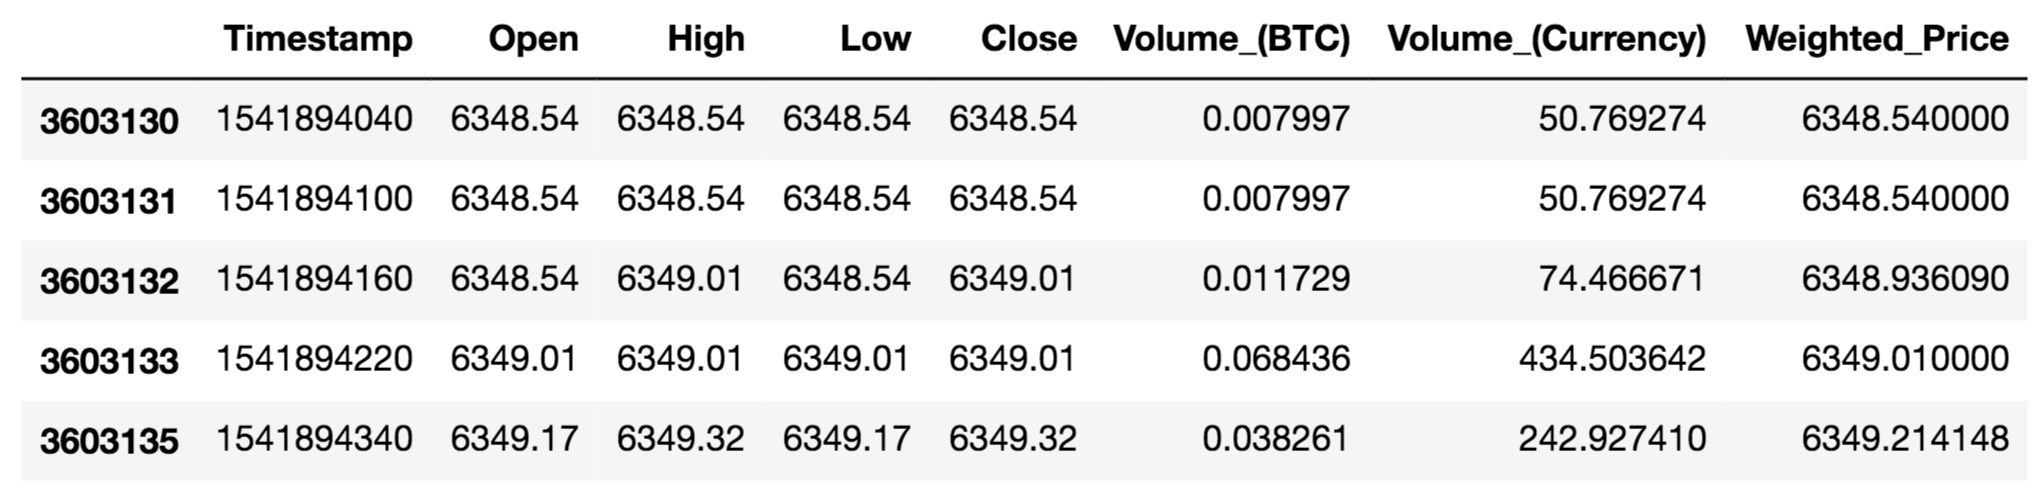
\includegraphics[width=0.9\columnwidth]{images/bitstamp-dataset.png}
\caption{Example entries from Bitstamp's BTC-USD dataset}
\label{fig:bitstamp-dataset}
\end{figure}

One well-known fact about cryptocurrency prices is their significant short- and long-term volatility. To have a stable basis to build on, given recent spikes and dips at the start of the year 2018, we chose to evaluate our models on the time period between 1st January 2016 and 20th October 2017. From this dataset, we only keep the price data daily aggregated, turning this into a univariate time series modeling and forecasting problem.

TODO: discuss seasonal decomposition, stationarity

\begin{figure}[h!]
\centering
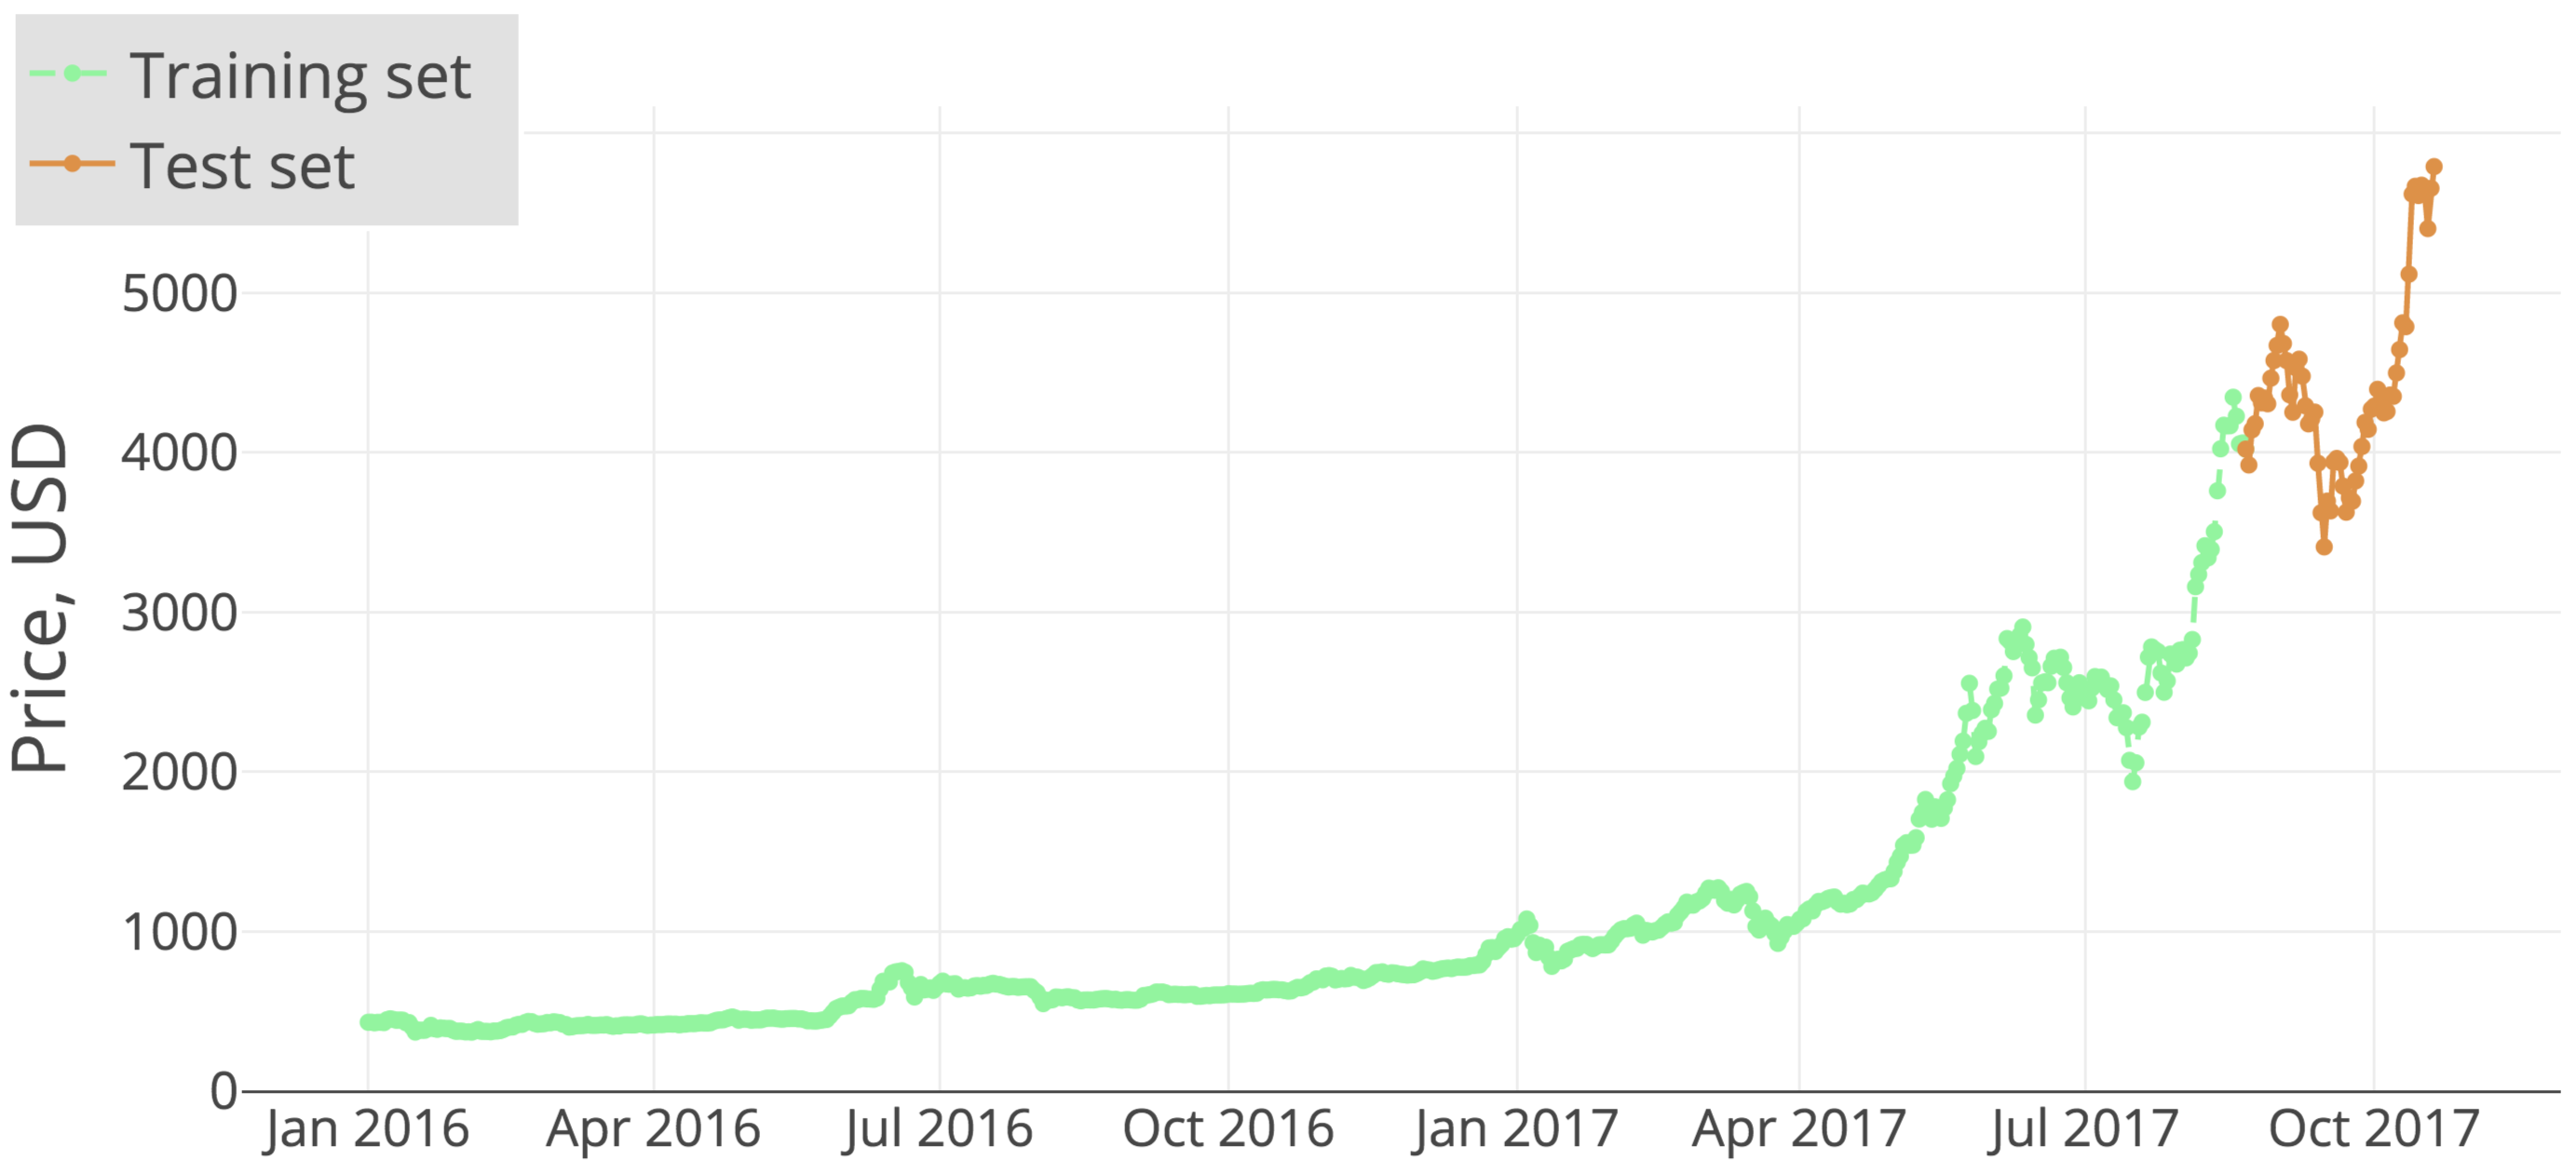
\includegraphics[width=0.9\columnwidth]{images/dataset.png}
\caption{Training and test sets during the chosen time period}
\label{fig:dataset}
\end{figure}

For separating the data into training and test sets, we tried two approaches.

\begin{enumerate}
    \item Choose a date and use it to cut the dataset into two (figure \ref{fig:dataset}). This is a common approach; however, the significant differences during different periods in our dataset might have a negative impact on the generalization ability of this approach.
    \item Cut the original dataset into \emph{chunks} of equal duration and then separate each of these into training and test sets. This approach will result in a more representative collection of data points. 
\end{enumerate}

TODO: add figure for second approach
TODO: compare these two approaches


\subsection{Introduction of models}

We used the following models for our evaluations:

\begin{itemize}
	\item \textbf{Linear regression}: In linear regression, we attempt to model the time-series using a linear model, basically fitting a trend line. It is a simple and fast model with limited generalization ability.
	\item \textbf{SVM regression (SVR)}: SVR is an extension of the SVM approach used for regression instead of classification. SVR maximizes the margin to derive a good linear regression model. Non-linearity can be introduced using kernel functions.
	\item \textbf{ARIMA}: Autoregressive Integrated Moving Average models are statistical models often used for modeling non-stationary time-series. 
	\item \textbf{LSTM}: Long Short-Term Memory is a type of Recurrent Neural Network (RNN), composed of cells including input, output and forget gates regulating the flow and retention of information.
\end{itemize}

A detailed theoretical discussion of these models is out of the scope of this paper.

TODO: add references

\subsection{Our approach}

Our work focuses on two distinct problems: single- and multi-step time-series forecasting. For both problems, we first define a simple baseline solution. Then, we proceed to implement a more complex, deep learning based approach using recurrent neural networks (RNNs). We compare the performance of these models with that of the baseline and discuss implementation details and challenges.

We decided to use the Root-Mean-Square-Error (RMSE) metric to compare our models. This metric is defined as the square root of the average squared error between the predicted values and the true labels of the training set.

$$\textrm{RMSE}(\mathbf{pred}, \mathbf{y}) = \sqrt{\frac1N \sum_{i=1}^{N} {(\mathbf{pred}[i] - \mathbf{y}[i])^2}} = \sqrt{\frac1N (\mathbf{pred} - \mathbf{y})^2}$$

For the implementation, we use common Python frameworks including numpy, pandas, sklearn, and keras. We rely on plotly for plotting.

The rest of the paper is organized as follows. In section \ref{sec:single}, we discuss the problem of single-step prediction, comparing LSTMs with a simple lag predictor (to be defined in \ref{sec:single-baseline}). Section \ref{sec:multi} turns to multi-step prediction. We compare and evaluate multiple baseline candidates in \ref{sec:multi-baseline}, and then proceed to apply LSTM to multi-step forecasting in \ref{sec:multi-lstm}. Section \ref{sec:eval} contains a general discussion of the results. Finally, we present related work in section \ref{sec:related} and summarize our results in section \ref{sec:conclusion}.


\section{Single-step prediction}
\label{sec:single}

\subsection{Problem definition}

First, let us define the problem of single-step prediction. In this scenario, we are given a time window of the last $n$ values of a time-series. Our goal is to predict the value in the next time step immediately after this window.

$$\textrm{single\textnormal{-}pred}(a_1, a_2, ..., a_n) \approx a_{n+1}$$

An example of this approach is predicting tomorrow's price based on the last 7 days.

\subsection{Preprocessing}

As the problem definition suggests, single-point prediction is a supervised learning task, where our dataset consists of input windows and the corresponding labels.

$$\mathbf{x_i} = [a_{i+1}, a_{i+2}, ..., a_{i+n}] \hspace{2em} y_i = a_{i+n+1} \hspace{2em} i \in [0,N-n-1]$$

As our predictions are based solely on the price, $\mathbf{x_i}$ is a vector and $y_i$ is a scalar. (Another option would be to use more features, in which case $\mathbf{x_i}$ would become a matrix and $y_i$ would be a vector.)

We use a simple Python function to decompose our original time-series into a series of such $\langle\mathbf{x_i}, y_i\rangle$  pairs. This is basically a sliding window approach, with overlaps between the windows.

\subsection{Baseline}
\label{sec:single-baseline}

Our baseline for single-step prediction is a lag predictor: We simply assume that the price has not changed since the last day. 

\vspace{-1.2em}
$$\textrm{baseline}_{single}(\mathbf{x_i}) = \mathbf{x_i}[n] = a_{i+n}$$

Figure \ref{fig:single-baseline} shows the baseline for our sample dataset. At first sight, the predictions seem quite accurate. This is even more so if we evaluate this model on a bigger dataset: the two curves seem to fit perfectly. However, such visual evaluation is misleading, and that is why we rely on the RMSE instead. The RMSE of our baseline model on the test set is 161.024.

$$\textrm{RMSE}(\textrm{baseline}_{single}) = 161.024$$

\begin{figure}
\centering
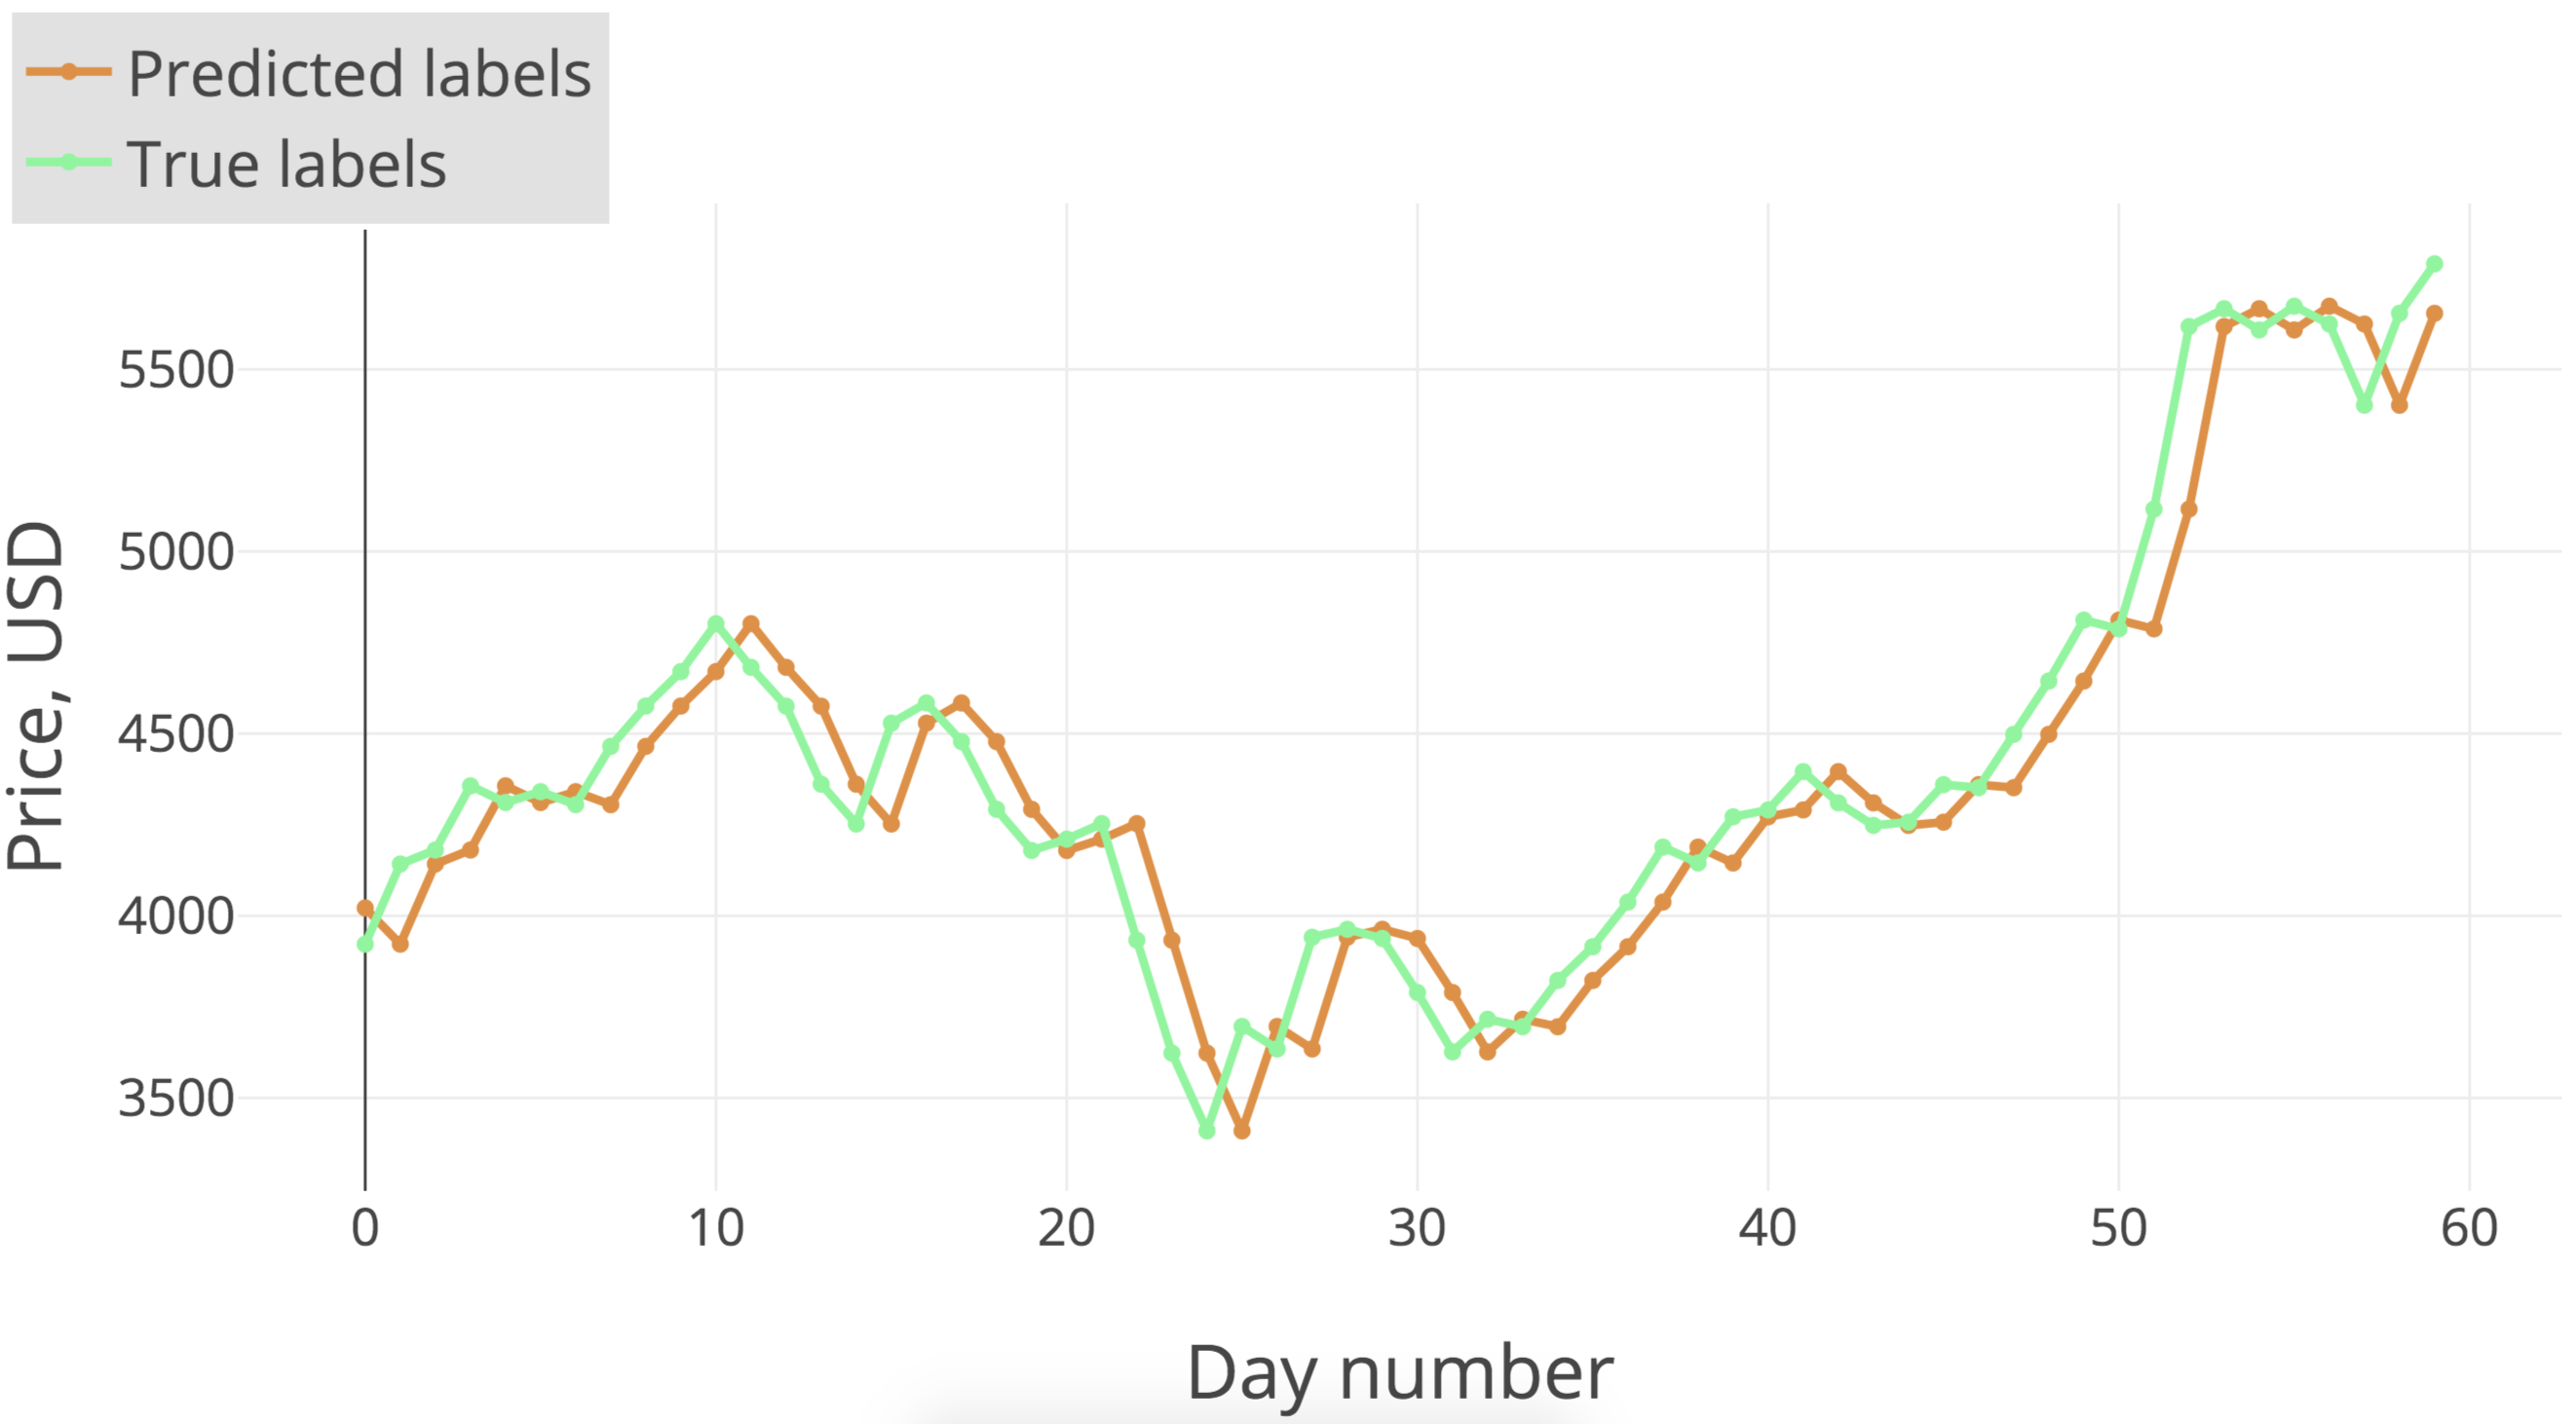
\includegraphics[width=0.9\columnwidth]{images/single-baseline.png}
\caption{Single-step lag predictor output}
\label{fig:single-baseline}
\end{figure}

\subsection{Model- and parameter-selection}

This first model we applied for the single-step problem was ARIMA. We tried different parameter configurations. The best results were delivered by an ARIMA(1,0,0) first-order autoregressive model.

$$\textrm{RMSE}(\textrm{ARIMA}_{single}) = 159.945$$

\begin{figure}[h!]
\centering
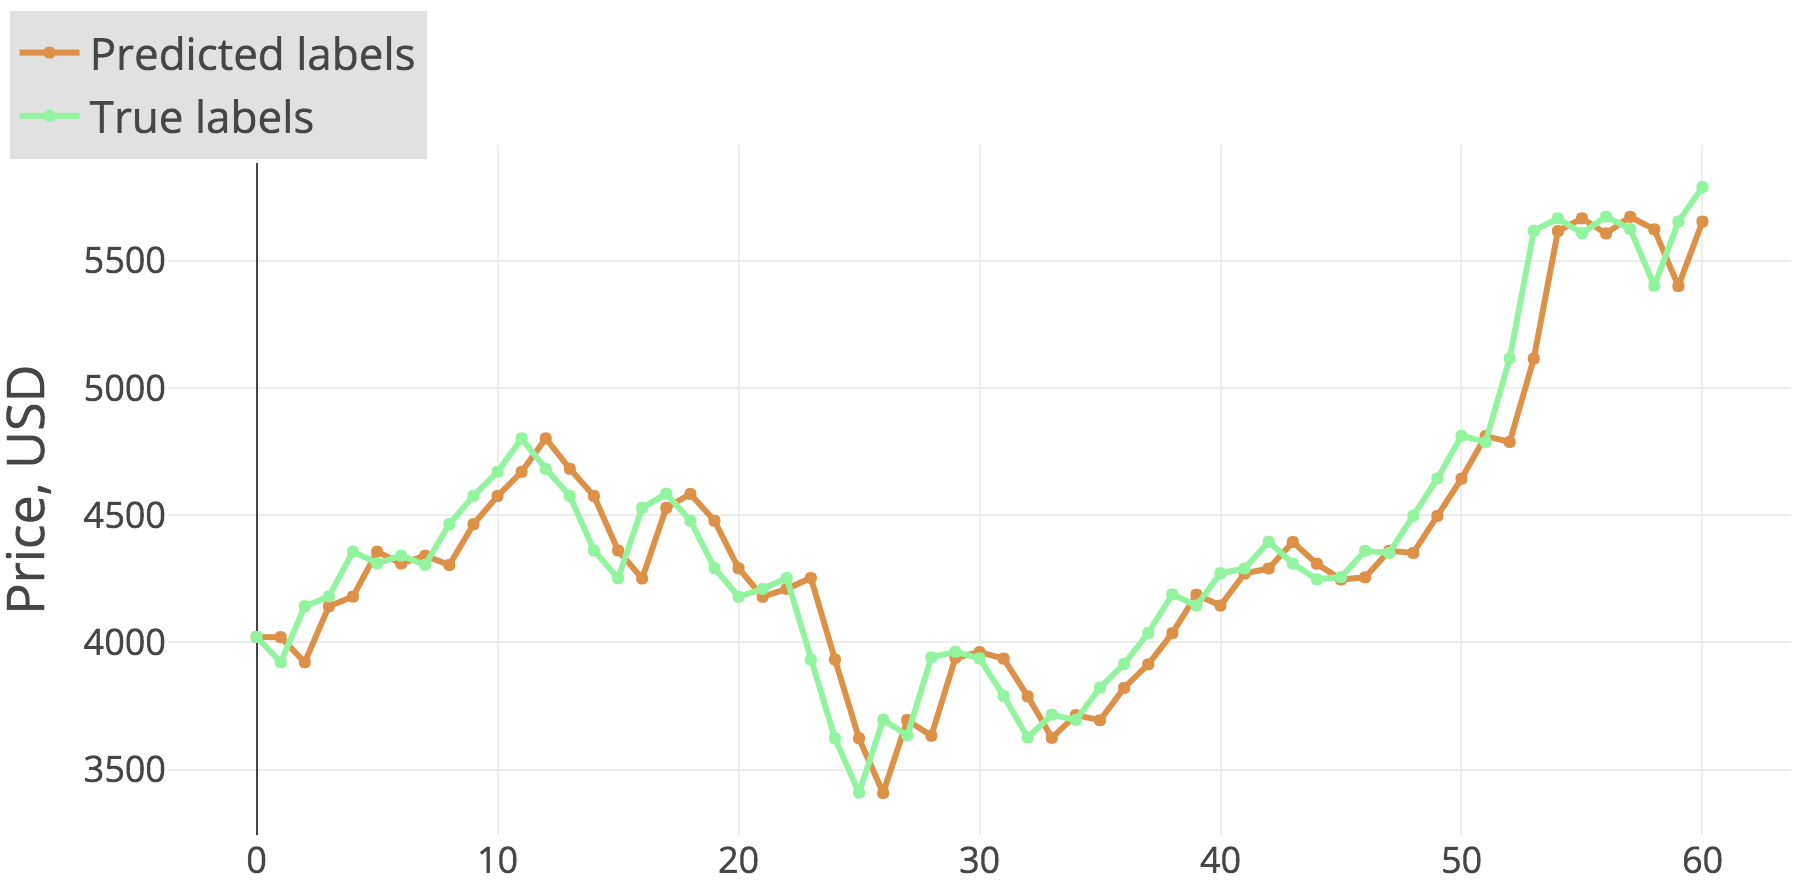
\includegraphics[width=0.9\columnwidth]{images/single-arima.png}
\caption{Example predictions using ARIMA}
\label{fig:single-arima}
\end{figure}

Next, we moved on to applying LSTM. After trying multiple network architectures, we found the best results were delivered by a network with 2 LSTM layers of 128 neurons each, with a densely connected output layer. (This network is very similar to the one used for multi-step prediction, illustrated by figure \ref{fig:lstm}.)

$$\textrm{RMSE}(\textrm{LSTM}_{single}) = 159.816$$

\begin{figure}[h!]
\centering
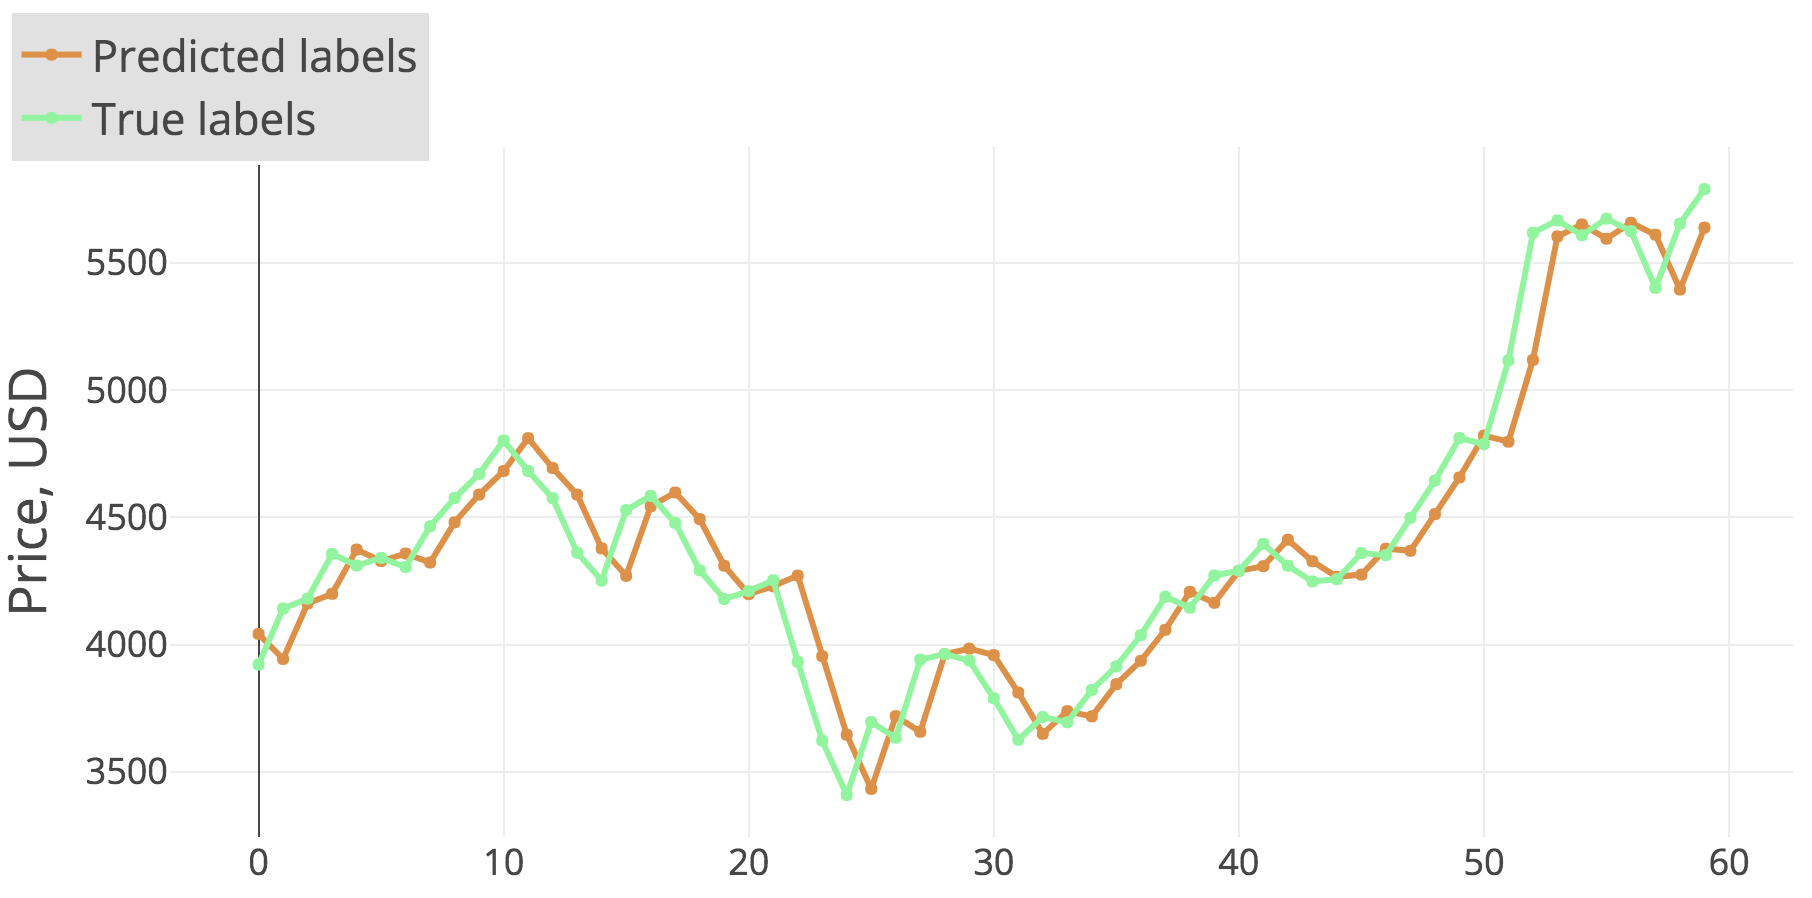
\includegraphics[width=0.9\columnwidth]{images/single-lstm-1.png}
\caption{Example predictions using LSTM}
\label{fig:single-lstm}
\end{figure}

\subsection{Results}

The RMSE of the different models evaluated (lag predictor, ARIMA, LSTM) shows no significant difference. This suggests that LSTM approximated the baseline but was unable to learn a better prediction based on the limited data available. Also given the simplicity of the prediction at hand, it would be hard to beat a simple solution.

TODO: add table/figure with RMSE

\section{Multi-step prediction}
\label{sec:multi}

\subsection{Problem definition}

In this section, we will present our results for multi-step prediction. In this scenario, we are given a time window (called \emph{look-back}) of the last $n$ price values. Our goal is to predict the price values for the next $m$ steps immediately after this window (called \emph{look-ahead}).

$$multi\textnormal{-}pred(a_1, a_2, ..., a_n) \approx (a_{n+1}, a_{n+2}, ..., a_{n+m})$$

An example would be predicting the next seven days' prices based on data from the past three weeks.

\subsection{Preprocessing}

Similarly to the single-point prediction problem, our dataset consists of input windows and the corresponding labels. The difference is that the labels in this case are also vectors and not scalars.

$$\mathbf{x_i} = [a_{i+1}, a_{i+2}, ..., a_{i+n}] \hspace{1.5em} \mathbf{y_i} = [a_{i+n+1}, a_{i+n+2}, ..., a_{i+n+m}] \hspace{1.5em} i \in [0,N-n-m]$$

Again, we rely on Python to decompose our original time-series into a series of $\langle\mathbf{x_i}, \mathbf{y_i}\rangle$ pairs.

\subsection{Baseline}
\label{sec:multi-baseline}

For choosing the baseline for multi-step prediction, we evaluated three models:

\begin{itemize}
	\item simple linear regression,
	\item SVM regression with radial basis function,
	\item ARIMA.
\end{itemize}

All of these models are applied to a single look-back window per prediction.

Figure \ref{fig:multi-naive} illustrates some example predictions of these three models. ARIMA delivered the best results during our evaluation, so we chose it as our baseline. As uncertainty grows with every step in multi-step prediction, the corresponding RMSE values are significantly higher than the single-step ones (figure \ref{fig:multi-rmse}). 

\begin{figure}[h!]
\centering
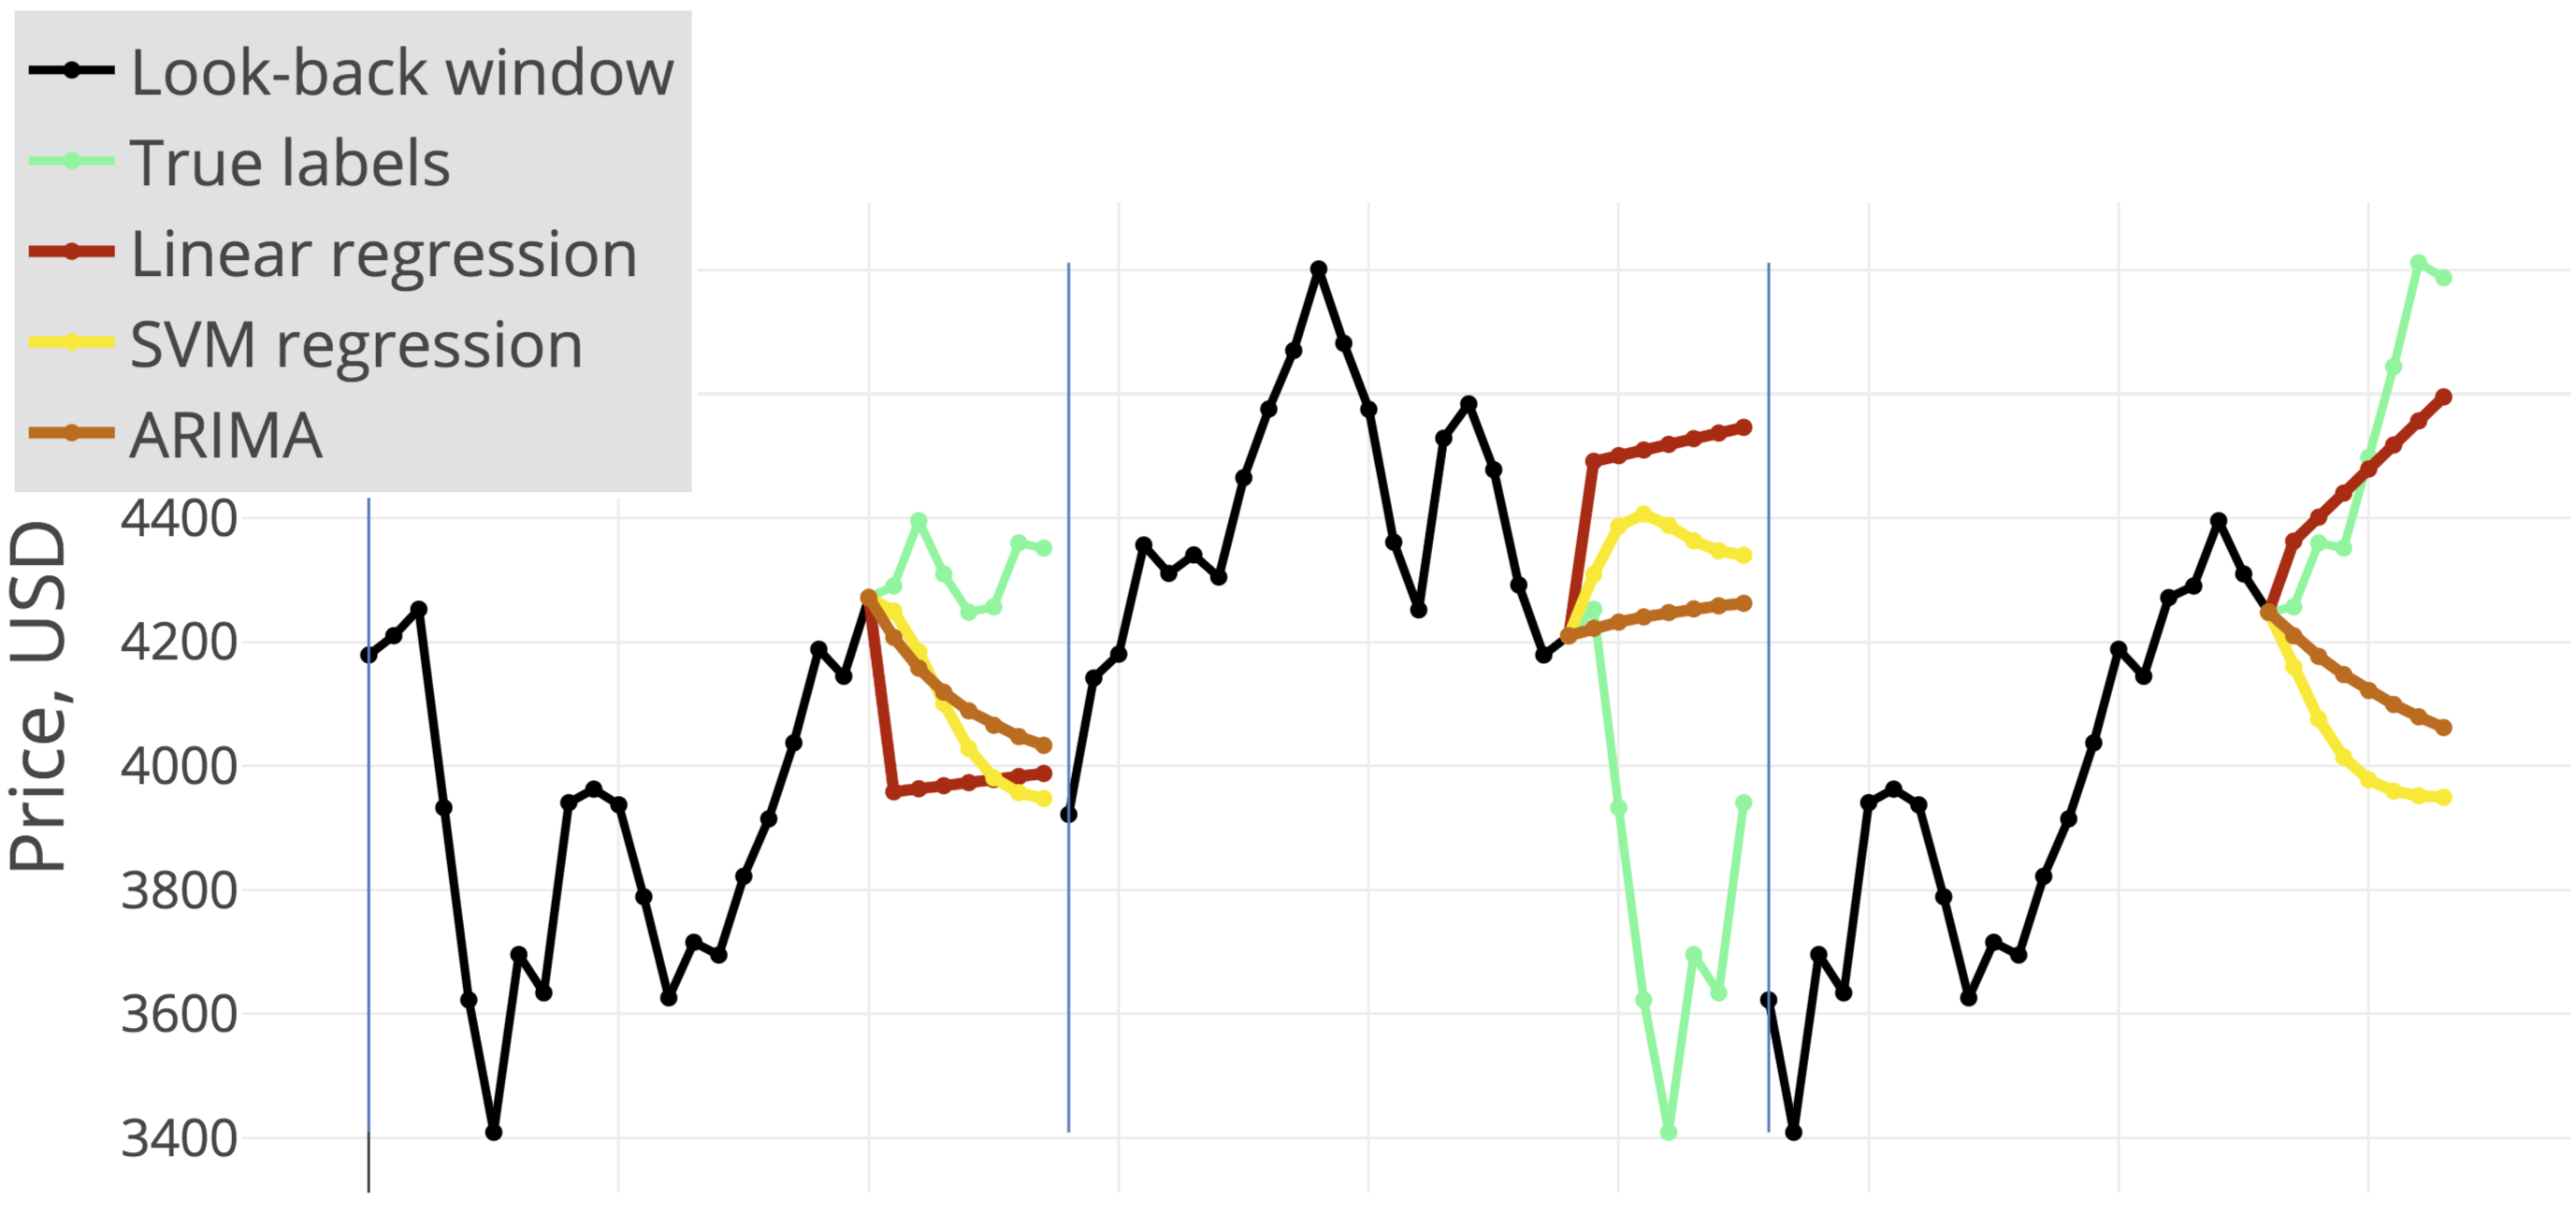
\includegraphics[width=0.9\columnwidth]{images/multi-naive.png}
\caption{Example predictions using the three baseline candidates}
\label{fig:multi-naive}
\end{figure}

\subsection{Model- and parameter-selection}
\label{sec:multi-lstm}

\begin{figure}[h!]
\centering

\includegraphics[width=0.4\columnwidth]{images/LSTM.png}
\caption{LSTM network parameters}
\label{fig:lstm}
\end{figure}

Our deep learning model for multi-step prediction is a deep LSTM network. The inputs are the look-back windows, while the outputs are the look-ahead windows.

Figure \ref{fig:multi-lstm} shows example predictions of our trained model.

\begin{figure}[h!]
\centering
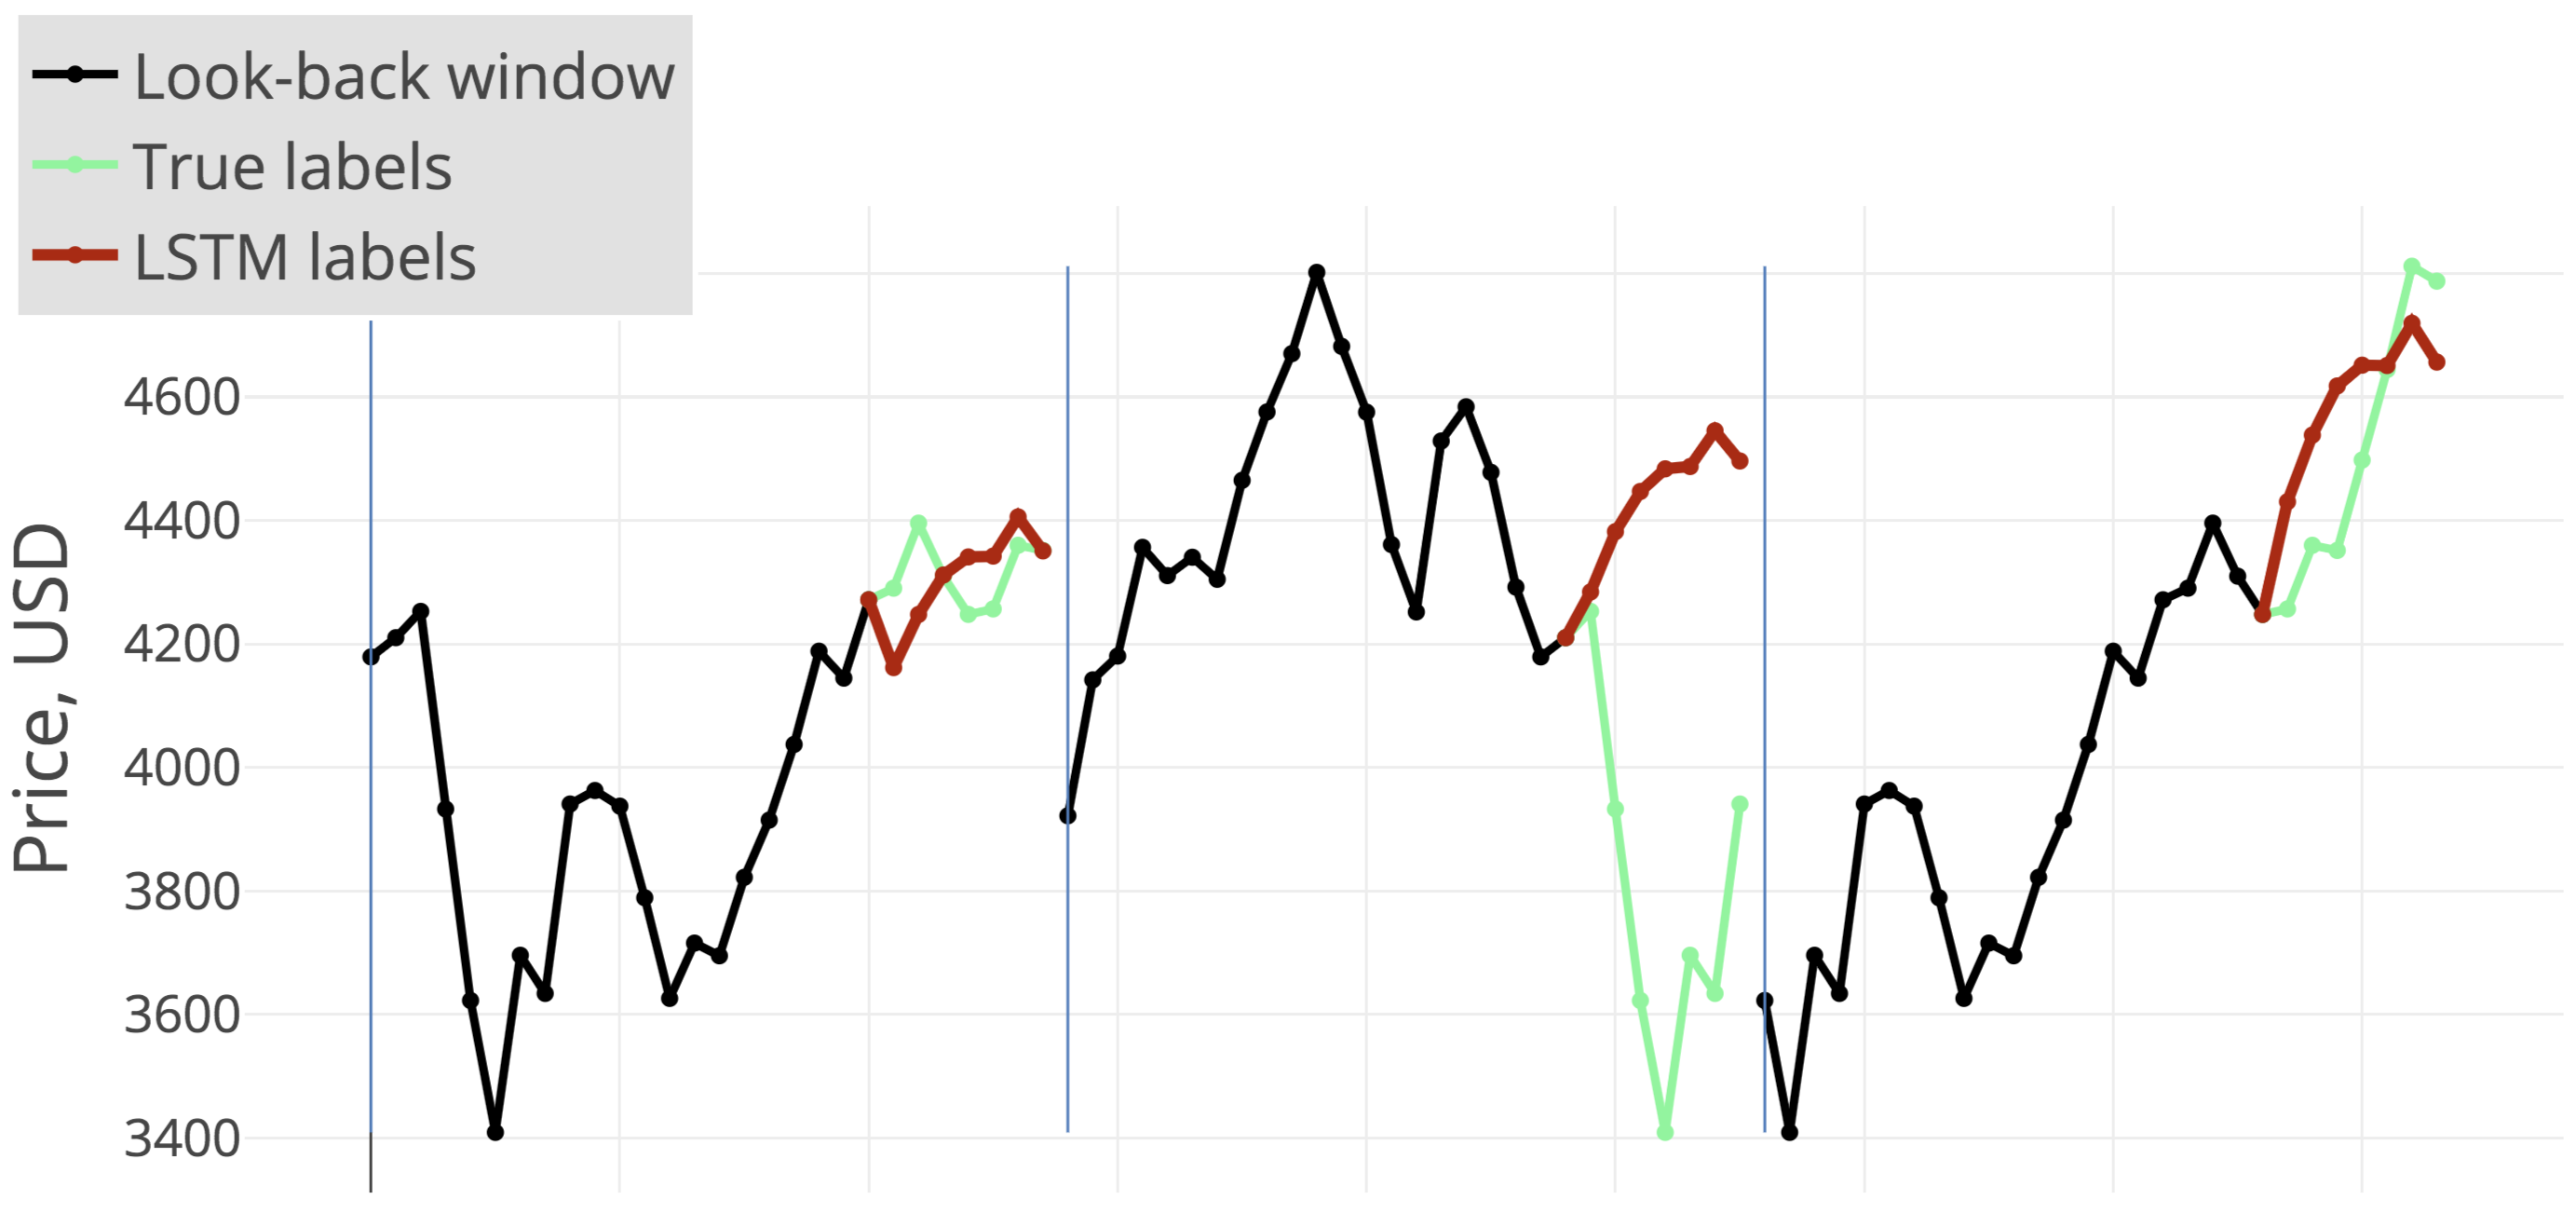
\includegraphics[width=0.9\columnwidth]{images/multi-lstm.png}
\caption{Example predictions using LSTM}
\label{fig:multi-lstm}
\end{figure}

\subsection{Results}

By using LSTM, we achieved a small but significant (about 9\%) improvement in overall prediction error on our test data. While these results rely heavily on the actual series being used, the results suggest that LSTM models can learn some complex changes automatically and thus outperform simple models.

\begin{figure}
\centering
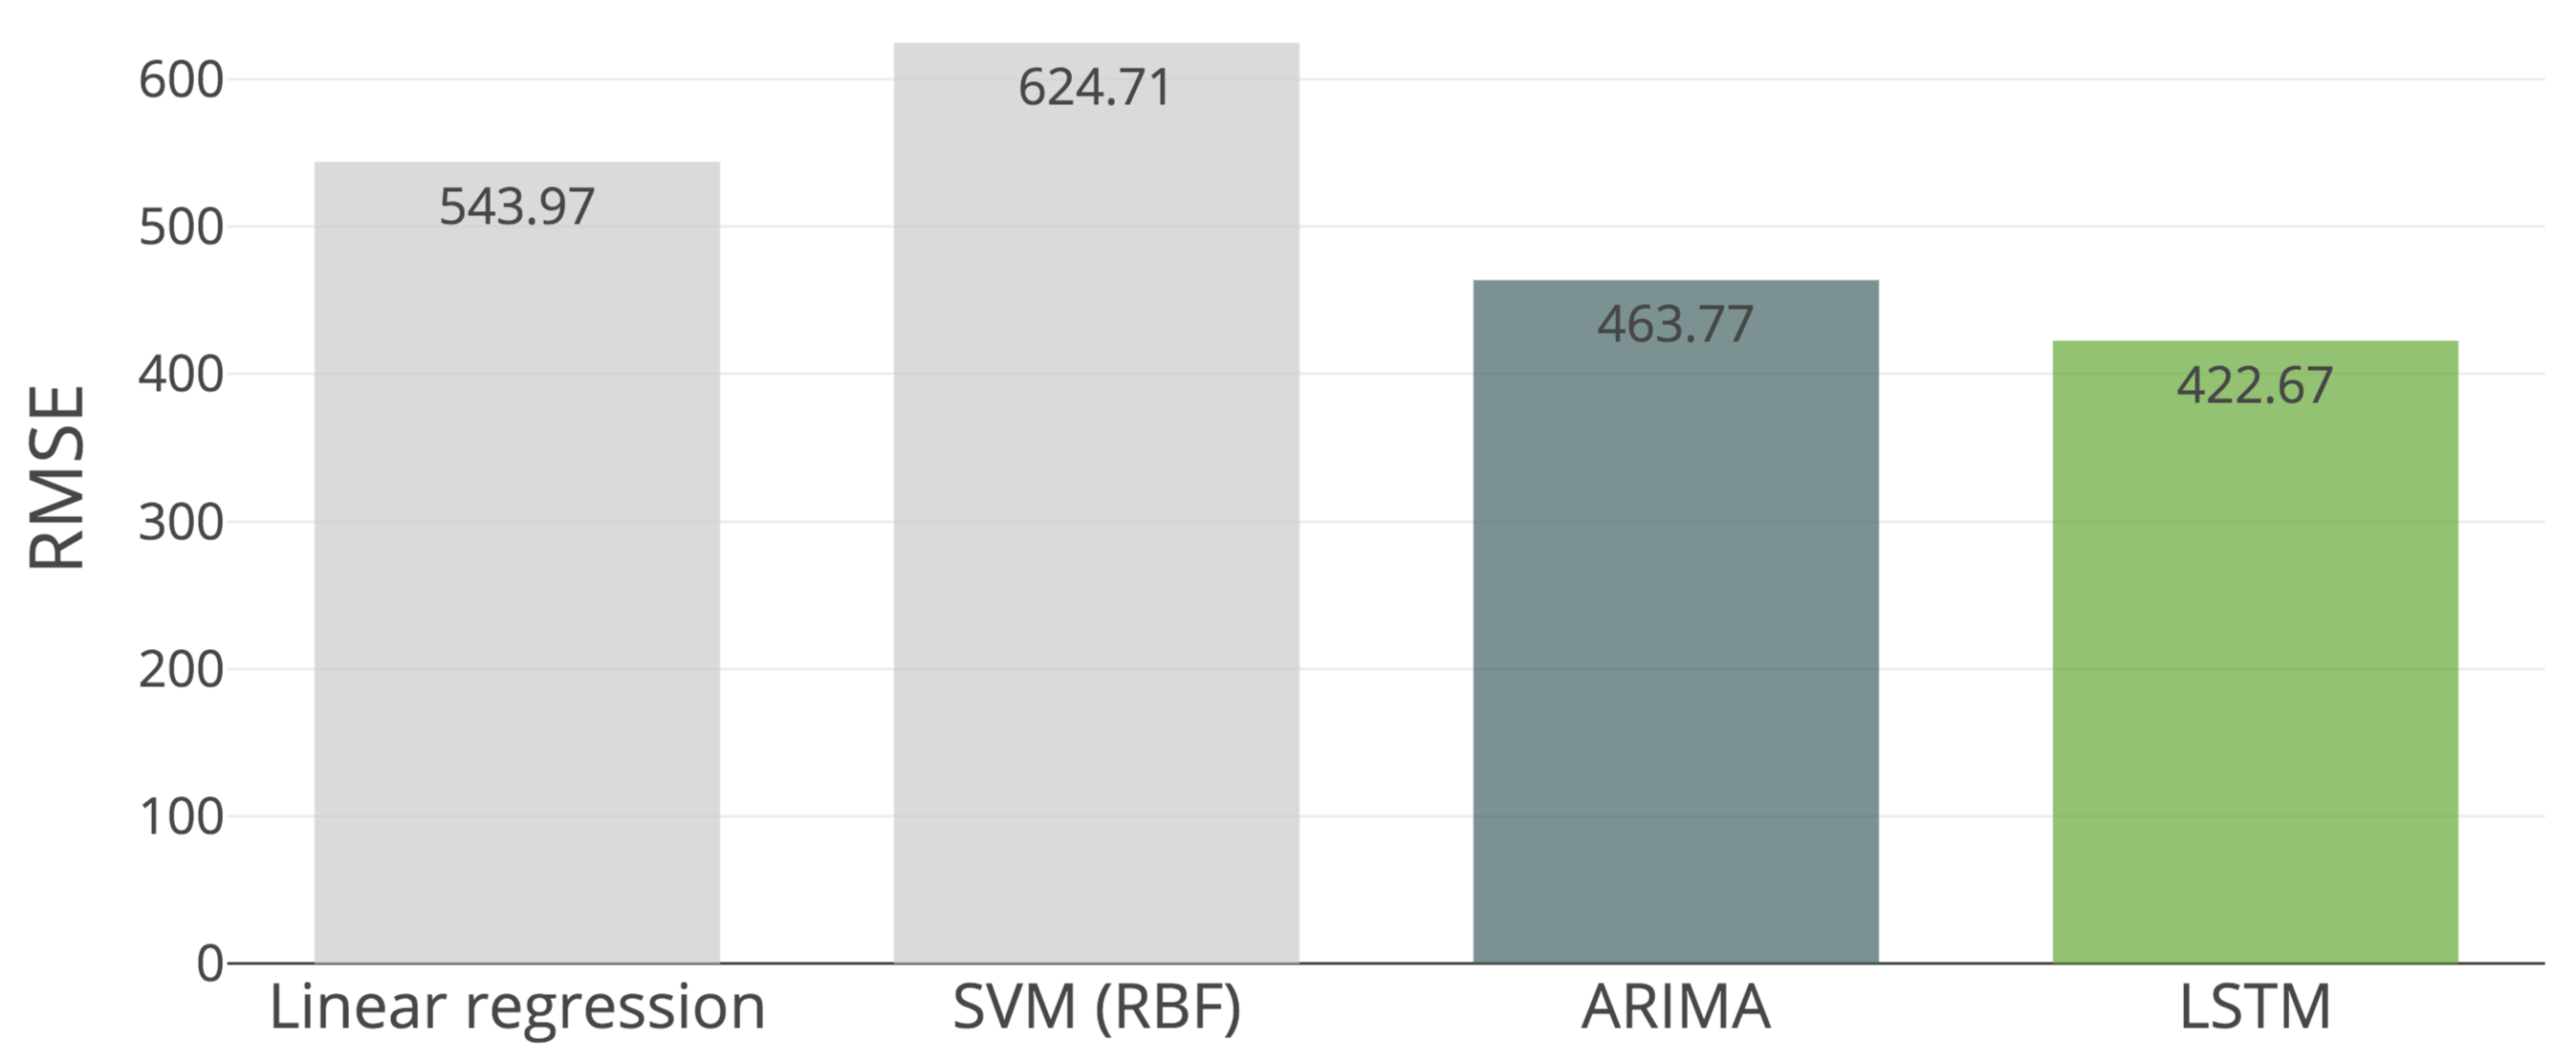
\includegraphics[width=0.8\columnwidth]{images/multi-rmse.png}
\caption{Comparison of prediction errors (RMSE)}
\label{fig:multi-rmse}
\end{figure}


\section{Evaluation}
\label{sec:eval}

\subsection{The impact of preprocessing}

\subsection{The impact of additional features}

\subsection{The impact of window size}

\subsection{The impact of network parameters}


\section{Related work}
\label{sec:related}

abc


\section{Conclusions}
\label{sec:conclusion}

\subsection{Overview}

We evaluated the use of LSTM for both single-step and multi-step time-series forecasting. For single-step prediction, using machine learning models offered no improvement compared to our simple baseline. For multi-step prediction, however, we achieved a \textasciitilde9\% improvement in prediction accuracy with LSTM compared to our best baseline ARIMA.

The results above suggest that the application of deep learning models for price prediction and other time series forecasting tasks is a promising area.

\subsection{Potential applications and use cases}

abc

\subsection{Future research directions}

Possible future directions for research include a more thorough evaluation of models, hyper-parameter tuning, incorporating more features into the models, and trying the same approaches on other datasets.


\section*{References}

\small

[1] Ariyo, Adebiyi Ariyo et al. (2014). Stock Price Prediction Using the ARIMA Model. 2014 UKSim-AMSS 16th International Conference on Computer Modelling and Simulation, 106-112.

[2] Chen, Kai et al. (2015). A LSTM-based method for stock returns prediction: A case study of China stock market. 2015 IEEE International Conference on Big Data (Big Data), 2823-2824.

[3] Hochreiter, S., \& Schmidhuber, J. (1997). Long Short-Term Memory. Neural Computation, 9, 1735-1780.

[4] Drucker, H., Burges, C.J., Kaufman, L., Smola, A.J., \& Vapnik, V. (1996). Support Vector Regression Machines. NIPS.

\end{document}
